\section{Experiments}

In order to properly study and select the different configurations, it is
necessary to analyize the behaviour of the algorithm, when we modify one
parameter at a
time. An automated test was developed for this purpose, provided in the annex,
with which we run a set of tests, changing the number of individuals, the number of
generations, the percentage of elitism, and the balance of percentage of
mutation and crossover. Each test, in each city is run a total of 5 times,
and the average is what is taken into account. \\
After that, a set of tests, created from the results obtained in the general
set, is made, by selecting specific values. Both the general, and the specific
tests will serve as a medium to compare both representations, in order to look
for differences (or lack thereof)
\\
\subsection{General tests}
For the general tests, the default values are:

\begin{itemize}
  \item Number of individuals - 50
  \item Number of generations - 50
  \item Elitism - 0.05
  \item Crossover - 0.95
  \item Mutation - 0.05
  \item Stop percentage condition - 0.95
  \item Detection of loops on
\end{itemize}

And, the different values for each modified parameter are:

\begin{itemize}
  \item Number of individuals - [50,100,150,200,500,750,1000]
  \item Number of individuals - [50,100,150,200,500,750,1000]
  \item Elitism percentage - [0,0.05,0.1,0.2,0.5,0.75,1]
  \item Crossover|Mutation balance - [1|0,0.95|0.05,0.9|0.1,0.75|0.25,0.5|0.5,0.25|0.75,0|1]
 \end{itemize}

\subsubsection{Original code}

Due to space limitations, we will limit ourselves to only discuss the results
of the general tests, while refering to the correspondent graph in the
appendix. 

When it comes to number of individuals, as expected, a relatively low number
of individuals does not provide adecuate results, as can be observed by looking
at the start of the graph (4.13.1). Almost all datasets start in global maximum, and only
a couple in a local max. However, the majority of them have one of their
lowest point when the number of individuals is 200 (except for the highest
dataset, which has it's lowest point at 750) and from that point, it stays
constant, or even raises, hence it can be said that any number of individuals higher than 200
would not be benefitial, and actually be just cumbersome when it comes to
computational cost.

Regarding the number of generations (4.13.2), once again, it is to be expected that a
low quantity of generations will not yield good results. But that is not the
only thing the number of individuals and generations have in common, since it
seems like 200 is one of the best options for the number of generations.
There are some differences, for instance, at lower quantities of
generations, there is more fluctuation, and more datasets are positive
towards higher number of generations. In the specific tests this will be
further studied, whether 200, or a higher number is better, and whether the
higher associated computational cost is worth.

When it comes to the percentage of elitism (4.13.3), the results are clearer.
With no exceptions, the lowest value for every single one of the datasets
is between 0.05 and 0.1, any higher, or any lower, and the distance
skyrockets, having the highest distances values at elitism = 1. \\
This phenomena has an easy explanation, the higher the elitism, the more likely it is that the
algorithm will stay at a local maxima. \\

For crossover and mutation (4.13.4), the test reflects perfectly the balance between exploitation and
exploration, the overall result shows that the best performance comes when
mutation has a value of 0.5, and crossover 0.5.\\
Any value of mutation higher than 0.5, and the results start to worsen, because
there is too much exploitation, and too litle exploration. Any value of mutation
lower than 0.5, and the results, most of the cases, are far worse. This leads to
the conclusion that 0.5 is the candidate for the specific tests, alghouth
the nature of the result makes it necessary to test other values, since,
we think these results are a bit odd, hence we will further
study in the specific tests, in order to make a conclussion.

\subsubsection{Modified code}

As explained in the implementation section, the representation we
implemented is path representation. Again, we will only discuss the
results, the graphs can be found in the appendix

Similarly to adjacency representation, the result for the test (4.13.5)
of increasing the number of individuals has a generally located minimum local at
200, although for some cases, the distance becomes constant at 100. The only
noticeable difference is that the values for the distances when the number of
individuals is very high (750,100) does not increase, rather it seems to keep
ever so slightly decreasing.

With regards with number of generations(4.13.6), once again, as expected, there is a number of individuals from which the
change in the result is almost insignificant. That point, as can be observed, is 200
individuals, the same as the other representation. One difference is that the
values obtained from 750 individuals forward is actually worse in some
cases, if not the same, while with the other representation there were some
cases in which it improved.

For the elitism(4.13.7), there is no doubt that 0.05 is the best
percentage of elitism that can be choosen with this representation. The results
are somewhat similar to the previous representation, but the slope at the
latest values (0.5 forward) is not so steep

Lately, the result of the crossover and mutation (4.13.8)  test is daunting. It was repeated, in case it was somehow erroneous, but the same graph was obtained.
\\

\subsection{Specific tests}

The specific tests are separeted in 2 phases, the first one, studying the impact of the best parameter values seen in the general
tests, for each representation individually. When explainig the impact of the
second representation, our implementation, it will be compared to the first\\
All the tests have been made with the benchmark dataset called bcl380.tsp.

\subsubsection{Original code}

The base values are the same as with the general case.
\big[Number of individuals, generations, percentage of elitism, of crossover and
mutation] = [50,50,5\%,95\%, 5\%\big]

The result obtained is

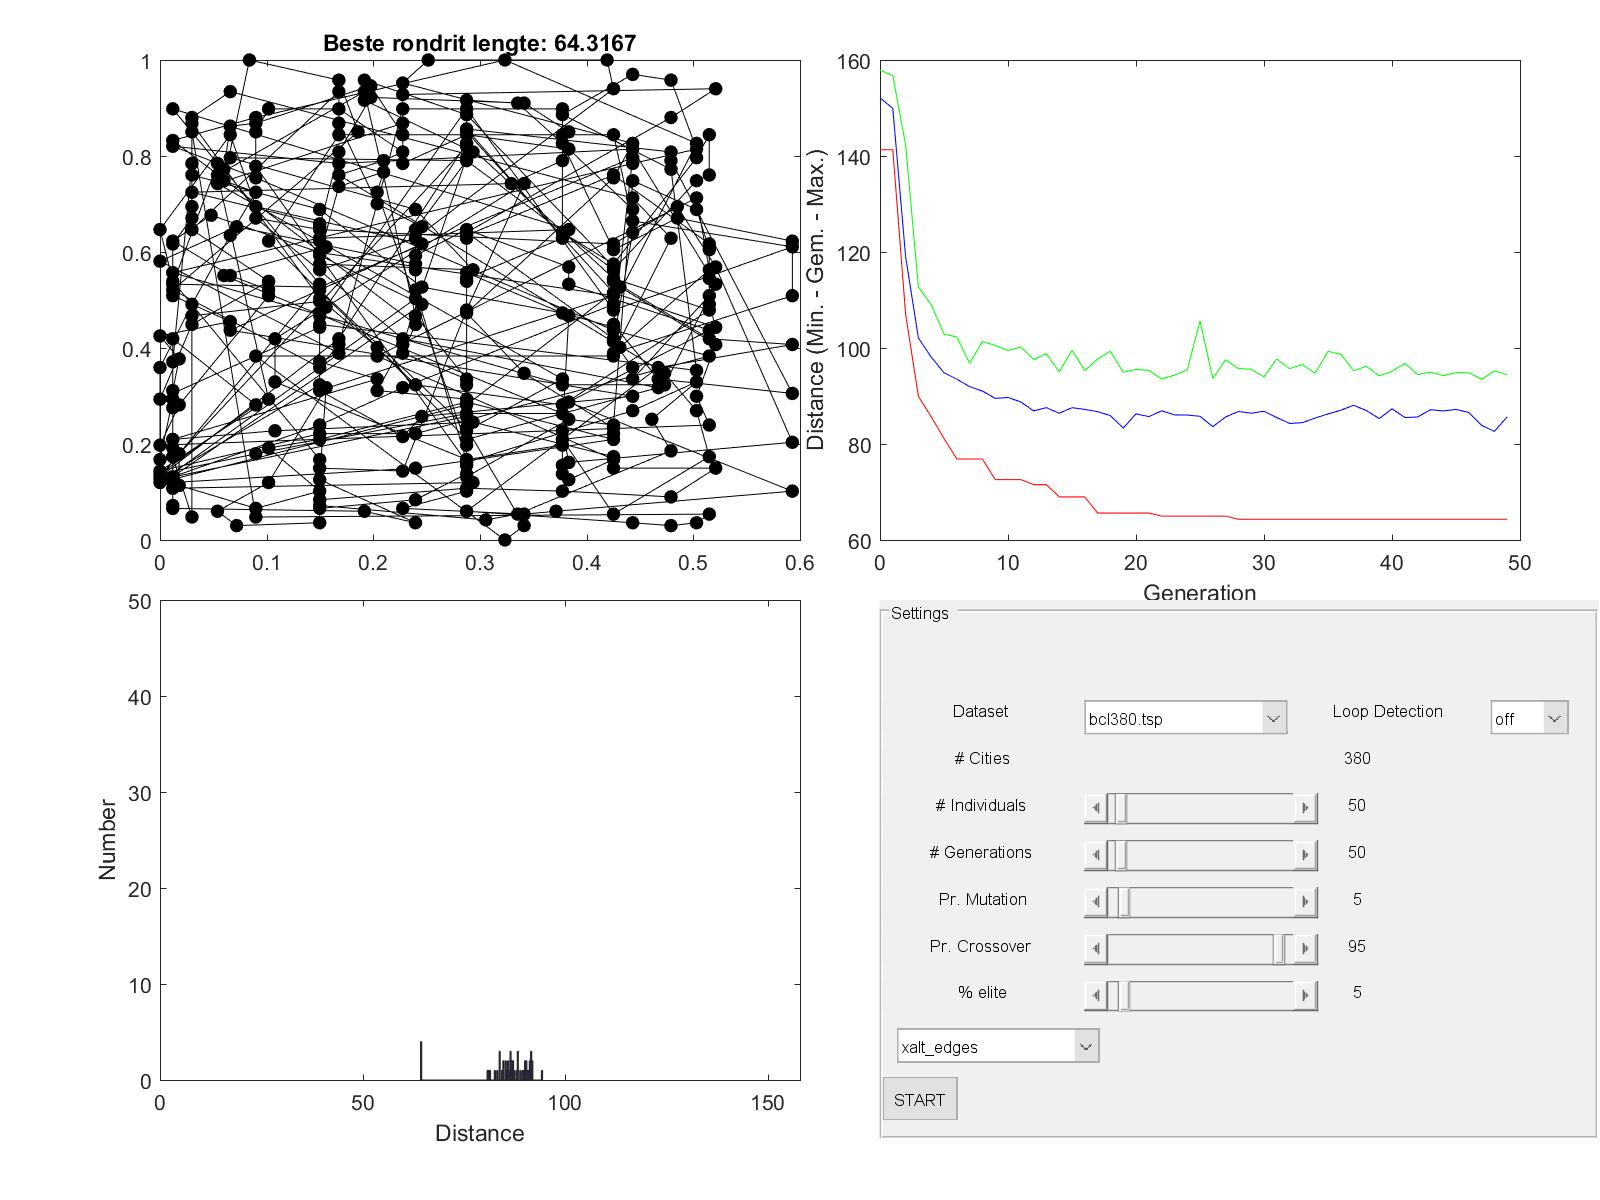
\includegraphics[width=13cm]{img/specific/xalt_edges/general_1.jpg}

The test was executed in 12.66 sec

200 was the number of individuals that was deemed to be apropiate. 
The test, keeping all other values, but changing just the number of
individuals is:
\\
\big[Nind, gens, elitism, crossover, mutation\big] =[200,50,5\%,95\%,5\%] \\
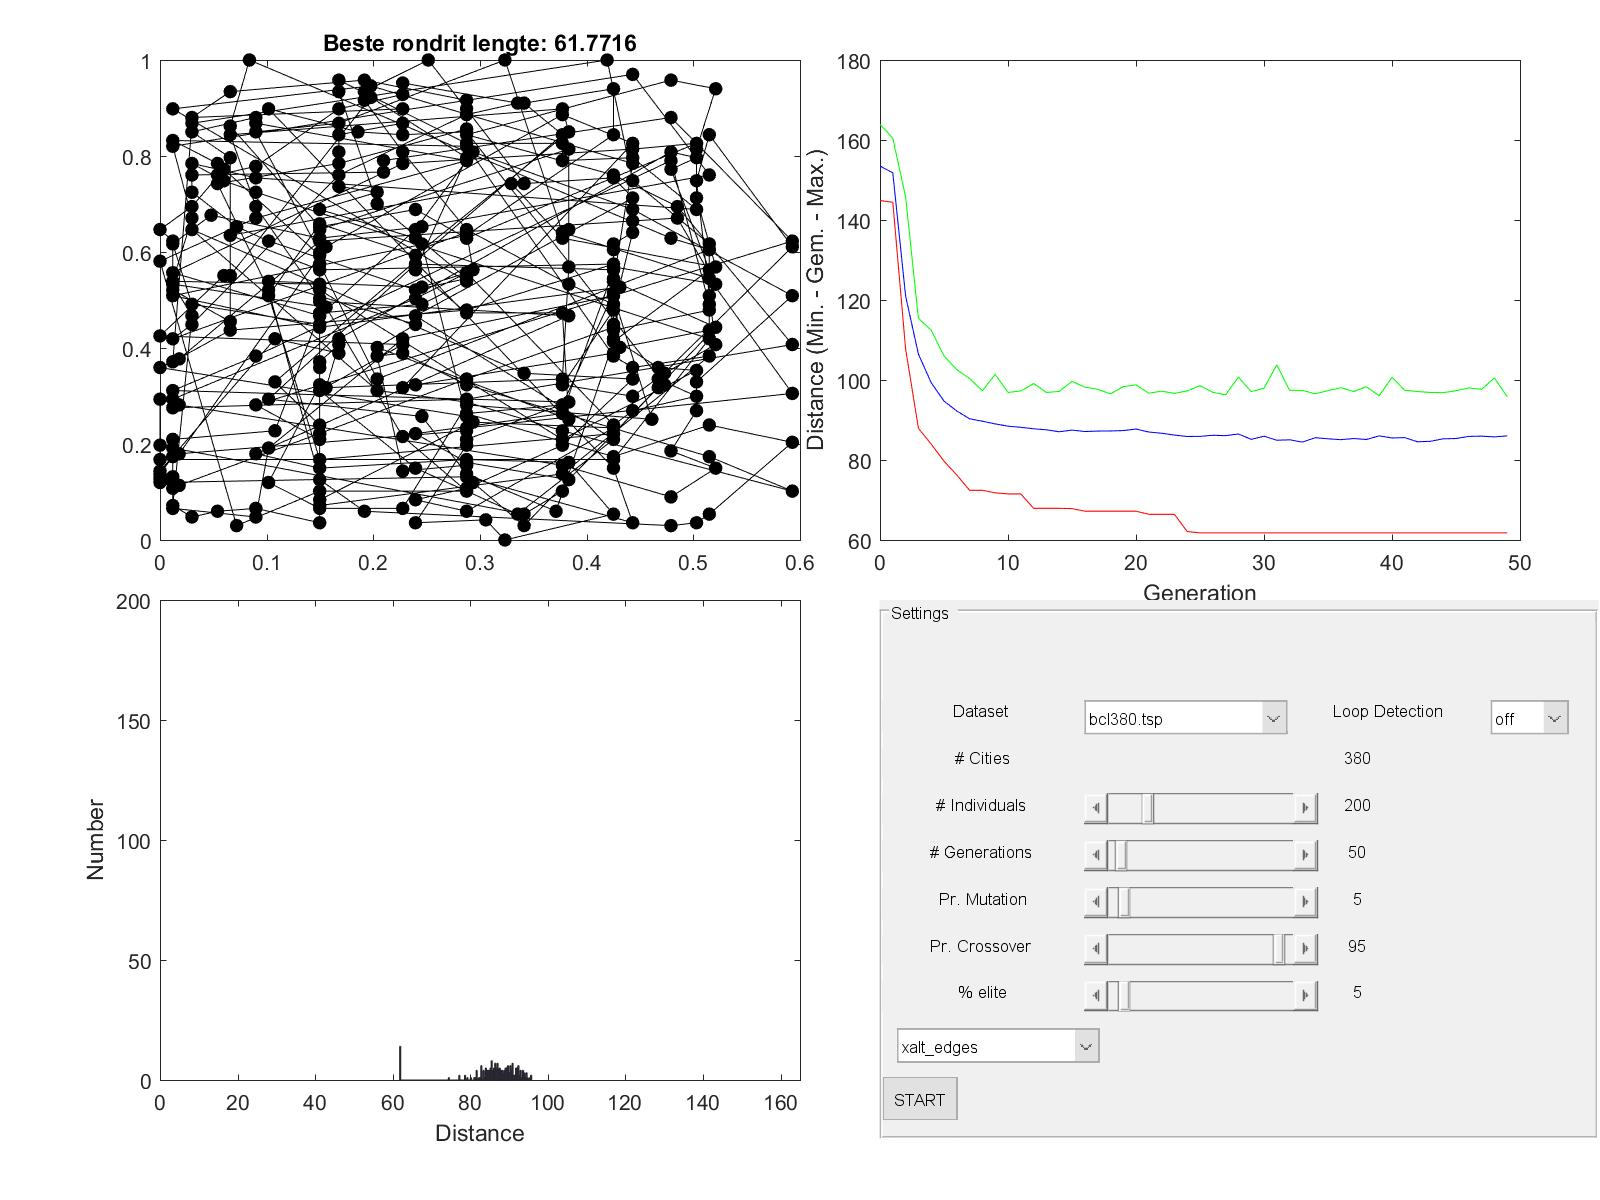
\includegraphics[width=13cm]{img/specific/xalt_edges/general_2.jpg}\\
We can see that the minimum distance has decreased, from ~64 to ~61, not a
big decrease, but significant enough. Increasing the number of
individuals to 200 is then to be considered a good measure. Timewise, the test was executed in 31.61 seconds. More than twice the time for the
first, which, given the increase in the number of individuals, is not out of
the expected. \\
\\
For the next test, this time the number of generations has been
increased. As previously stated, the best number was 200, but a higher number
was also suitable for some cases. We tried, respectively, with 200, 750, and
1000 generations, thus having\\

\text{\big[50,200,5\%,95\%,5\%\big]}
\hfill
\text{\big[50,750,50,5\%,95\%,5\%\big]} \\
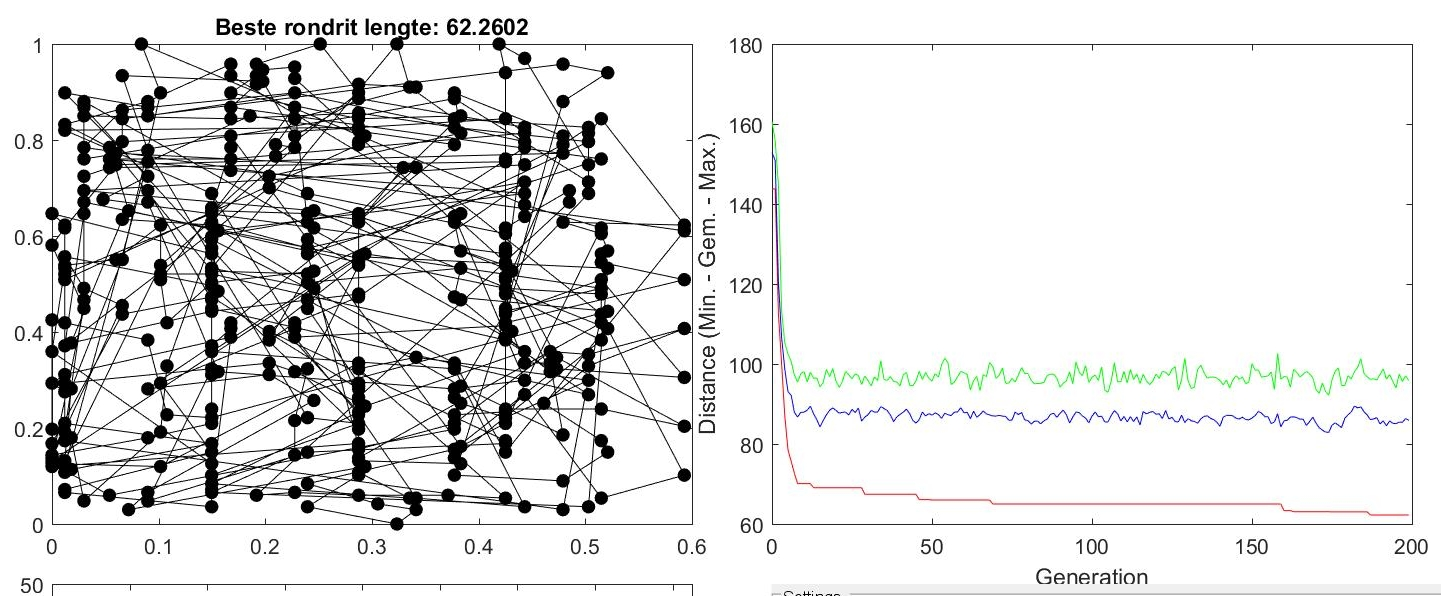
\includegraphics[width=9cm]{img/specific/xalt_edges/general_3.jpg}
\hfill
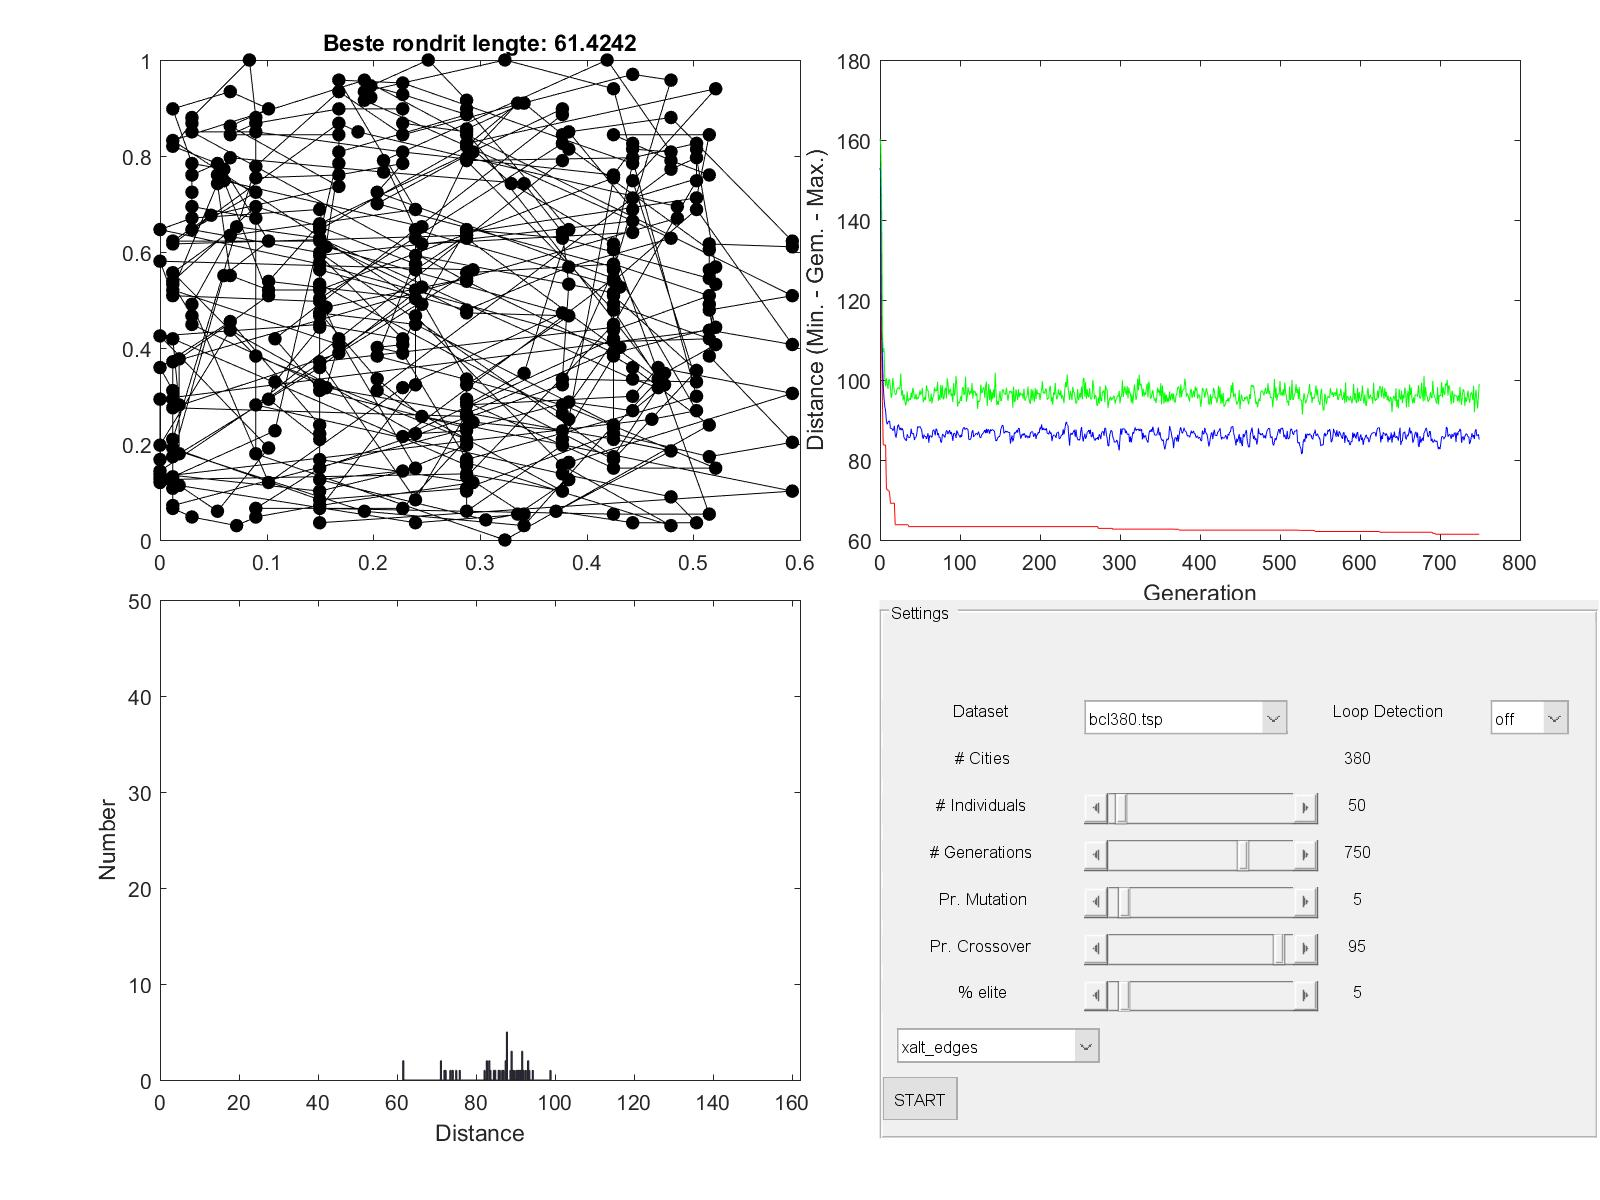
\includegraphics[width=9cm]{img/specific/xalt_edges/general_4.jpg}

\begin{center}
[50,1000,5\%,95\%,5\%]\\
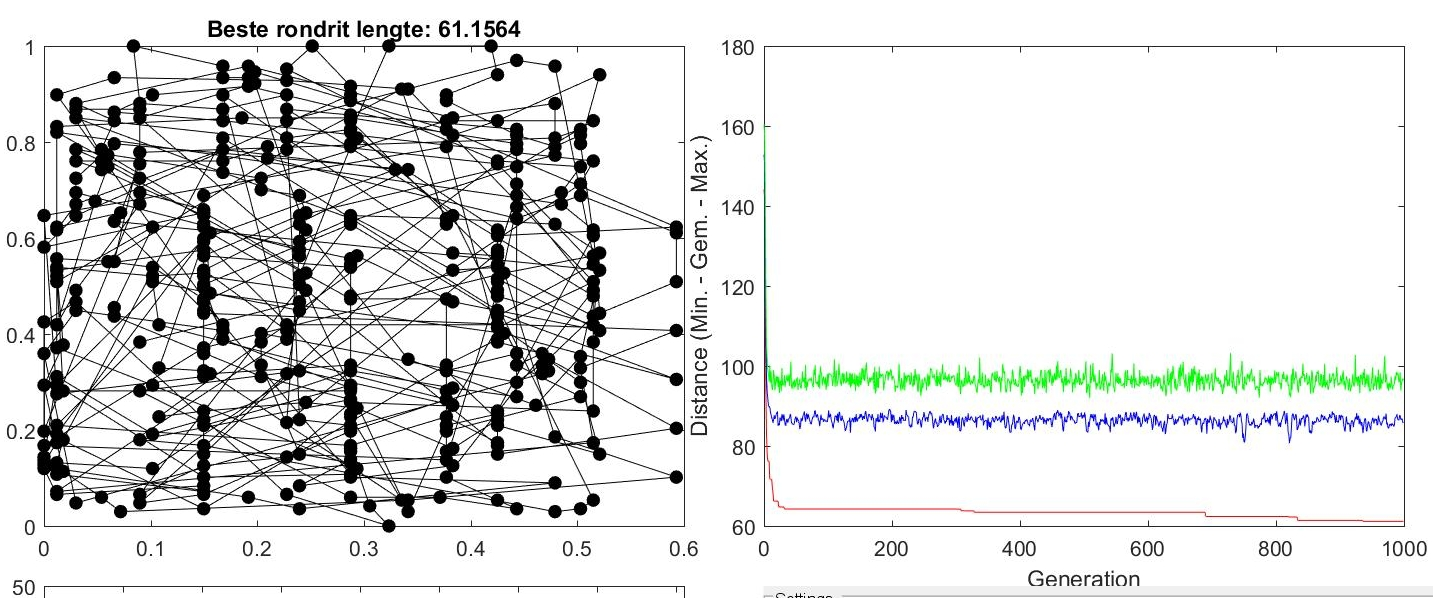
\includegraphics[width=13cm]{img/specific/xalt_edges/general_5.jpg}
\end{center}

We can observe that the result is slightly better, with each increment of
generations, but the cost is excesive, when it comes to time. The times for the
tests are 46.01, 171.67, and 233.85 seconds, which means, ~4, ~13.5 and ~18.5
times more than the base case.
\\
As the elitism parameter was abundantly clear that was to be kept at 0.05 (or
up to 0.1 at most), and it is already the value for the base case, there is
no specific test for the elitism. There is, however, for the percentage of
crossover and mutation. Since the result was a bit unexpected, we did not only
try with the apparent best result (0.5 percentage of each), but with cases of
0.2 crossover | 0.8 mutation, and viceversa. The results for the tests are\\
\newpage

\text{\big[50,50,5\%,50\%,50\%\big]}
\hfill
\text{\big[50,50,5,5\%,80\%,20\%\big]} \\
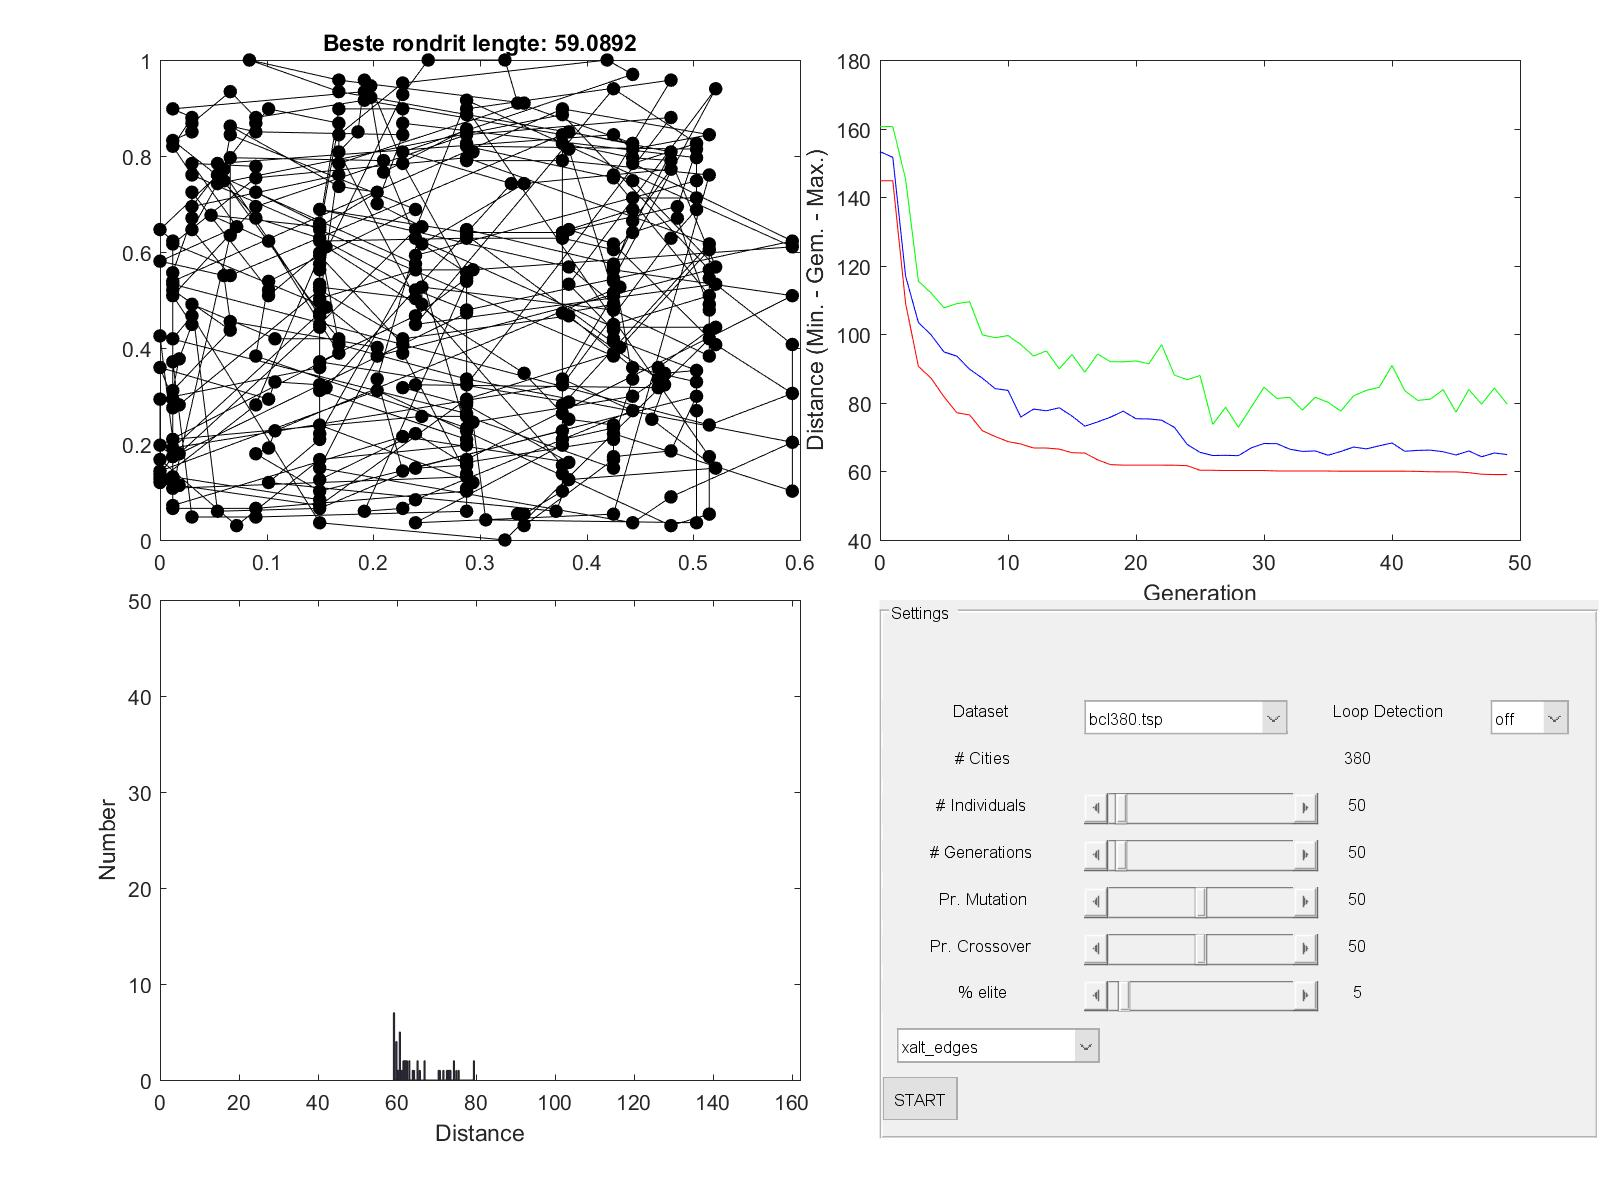
\includegraphics[width=9cm]{img/specific/xalt_edges/general_6.jpg}
\hfill
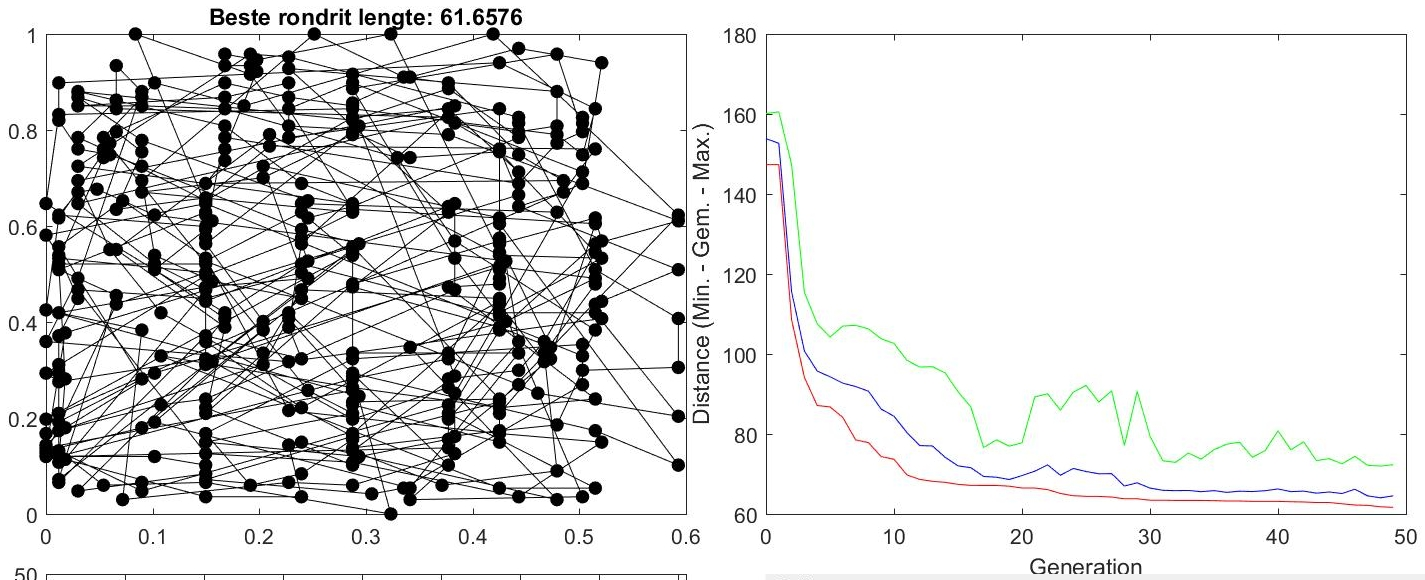
\includegraphics[width=9cm]{img/specific/xalt_edges/general_7.jpg}

\begin{center}
[50,50,5\%,80\%,20\%] \\
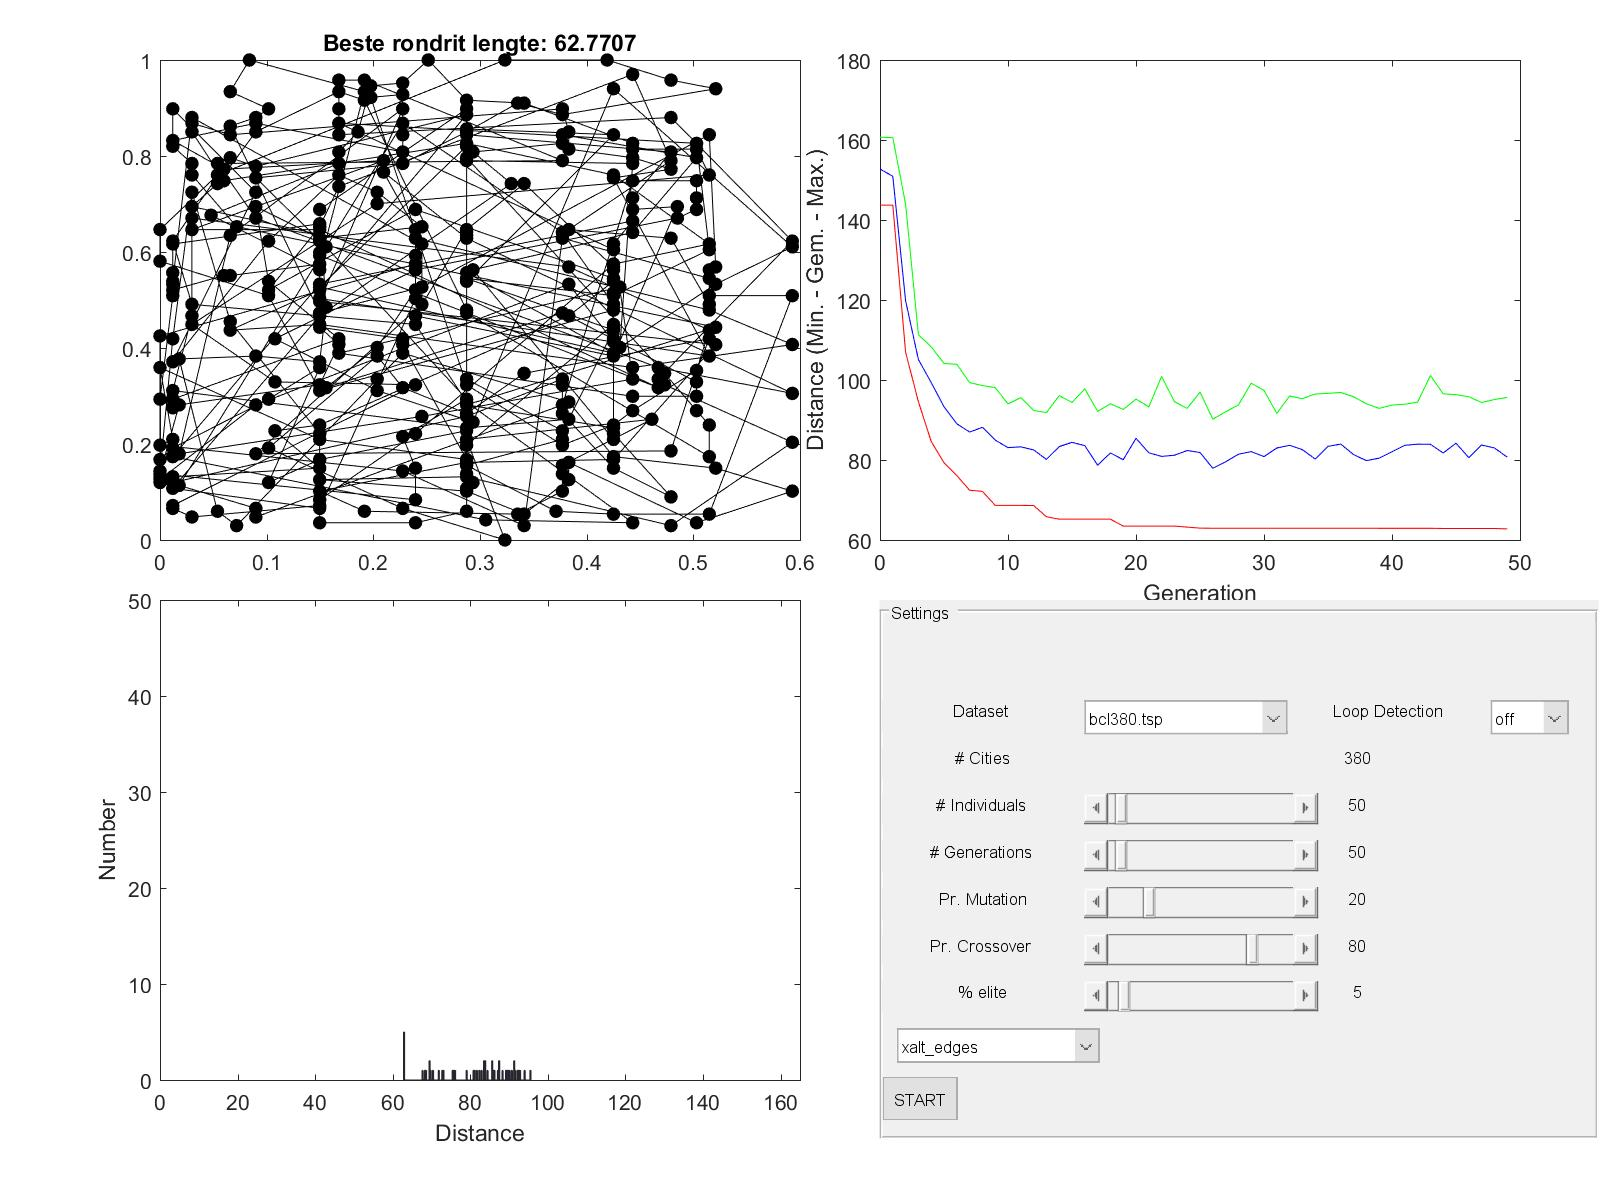
\includegraphics[width=13cm]{img/specific/xalt_edges/general_8.jpg}
\end{center}

The test confirms the results obtained in the general test. The best ratio of
crossover|mutation is 50\%|50\%, since, out of the 3 configurations, it has the
best result, while all of them are over the base case. Although not as relevant
in this case, the times of the tests are equal or even lower than the original, 11.3,
9.71, 12.92 seconds respectively. \\

Finally, the combination of the good results is what made them get
outstanding results. In order to avoid bias, the first combination is just
modifying the number of individuals, and the number of generations\\
\newpage
\begin{center}
[200,200,5\%,95\%,5\%] \\
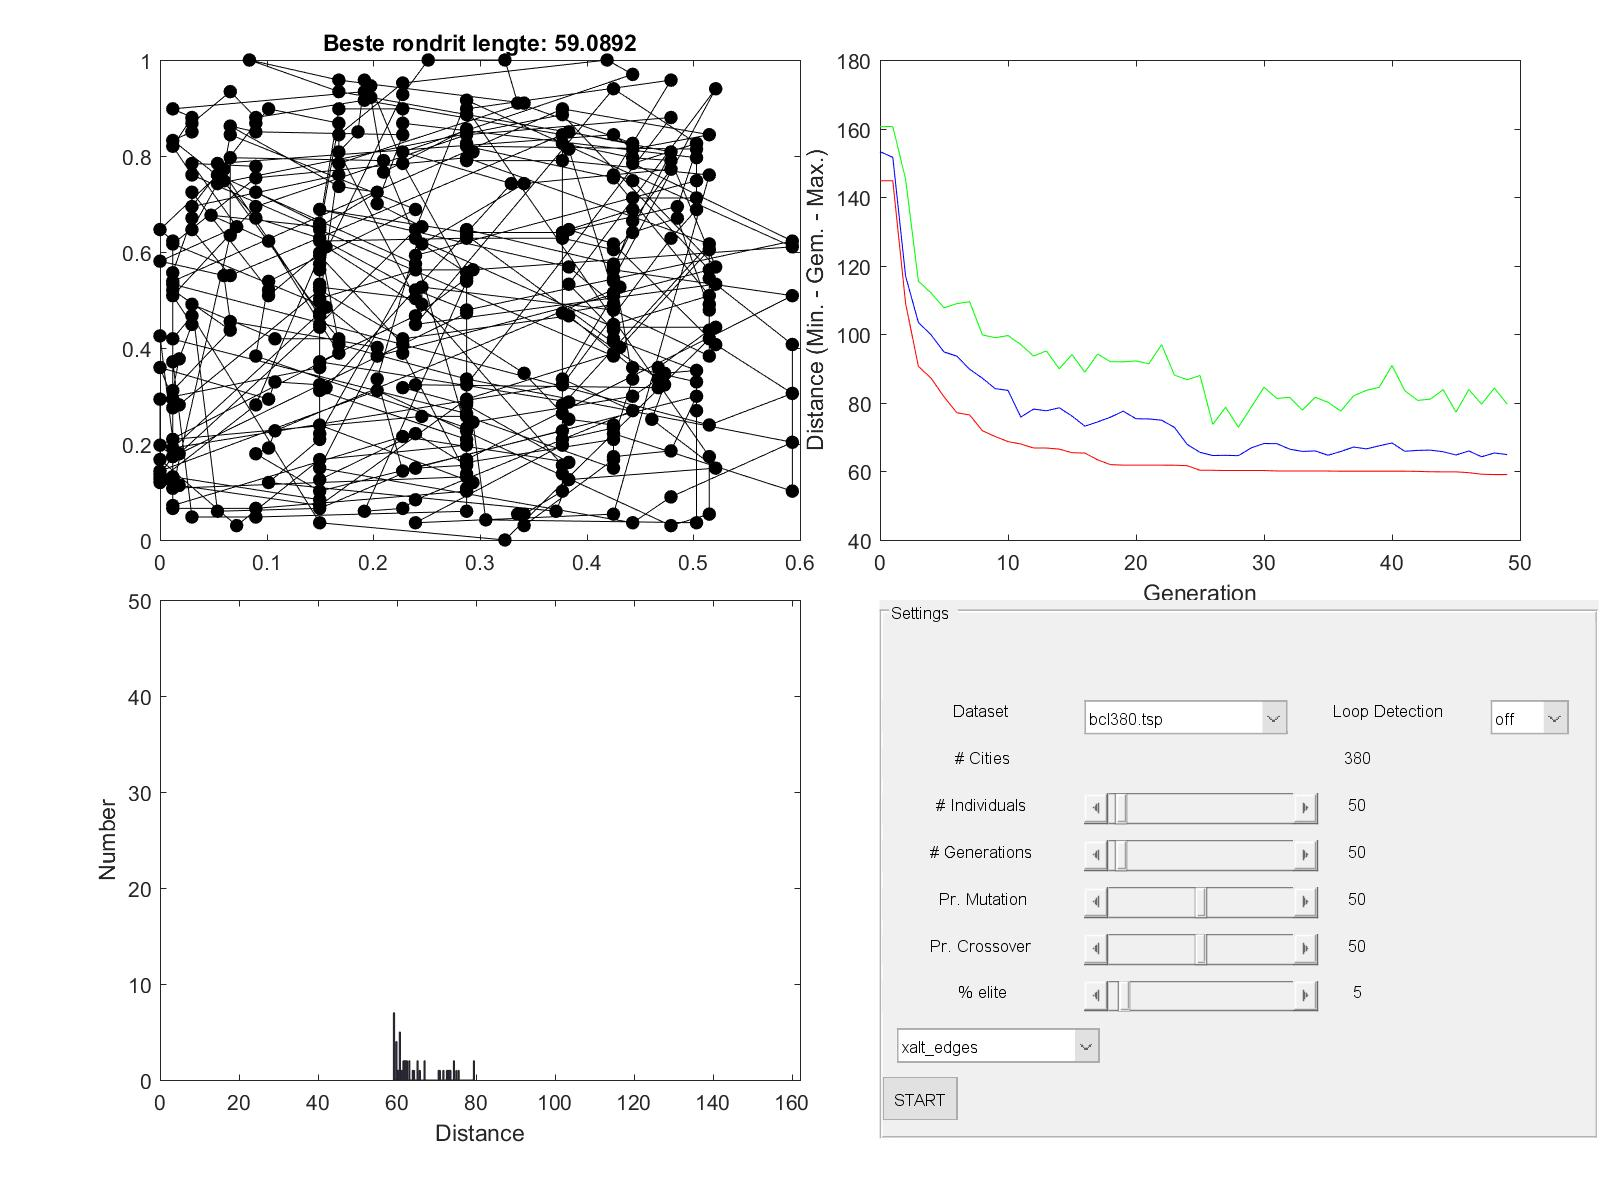
\includegraphics[width=13cm]{img/specific/xalt_edges/general_6.jpg}
\end{center}
We can see an improvement, even slightly better than those obtained with the
increase in number of individuals or generations alone. The number of
generations was choosen to be 200 because we deemed it good enough, and while
costly, not as costly as higher quantities.
\begin{center}
[200,200,5\%,50\%,50\%] \\
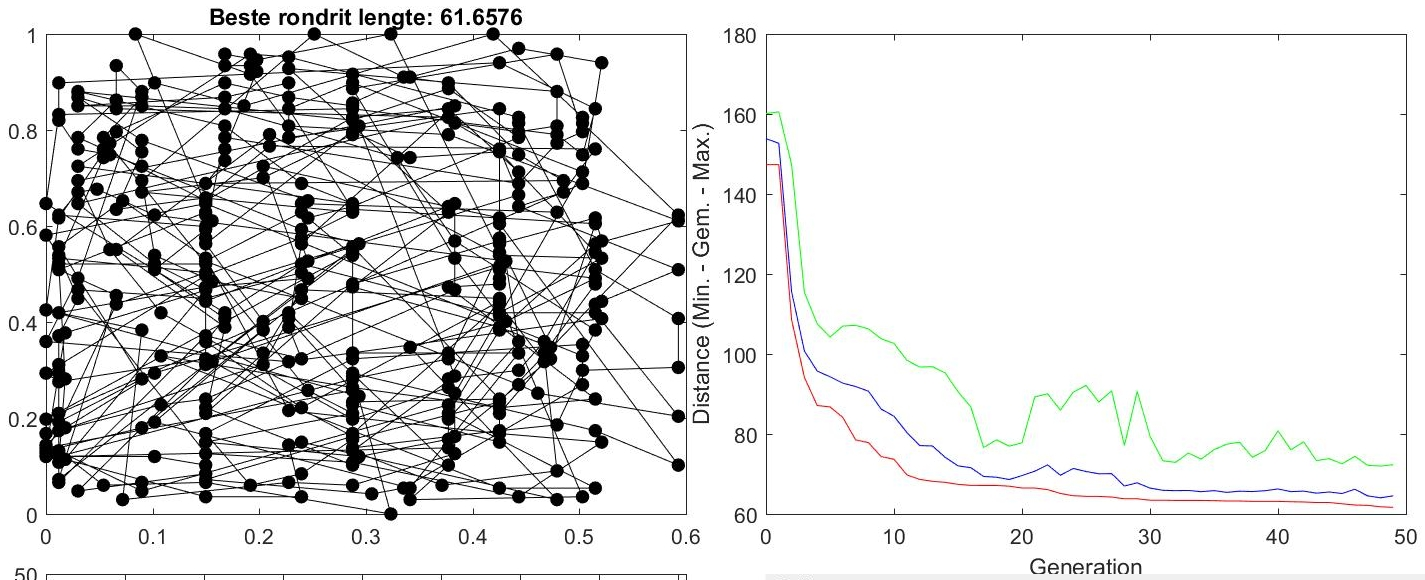
\includegraphics[width=13cm]{img/specific/xalt_edges/general_7.jpg}
\end{center}
And the final result, when combining every single improvement, is the best of
all. The decrease of distance is ~30.8\%, which could be said to be a great
decrease. The time spent on this test was 76.74 seconds, around 6.1 times
more than the original, although high, we consider that it is not
sufficiently high as to consider it bad. \\

\subsubsection{Modified code}

The same structure as the previous representation will be followed. One
parameter at a time will be tested, stating the change, after
performing a base test
\begin{center}
[50,50,5\%,95\%,5\%]\\
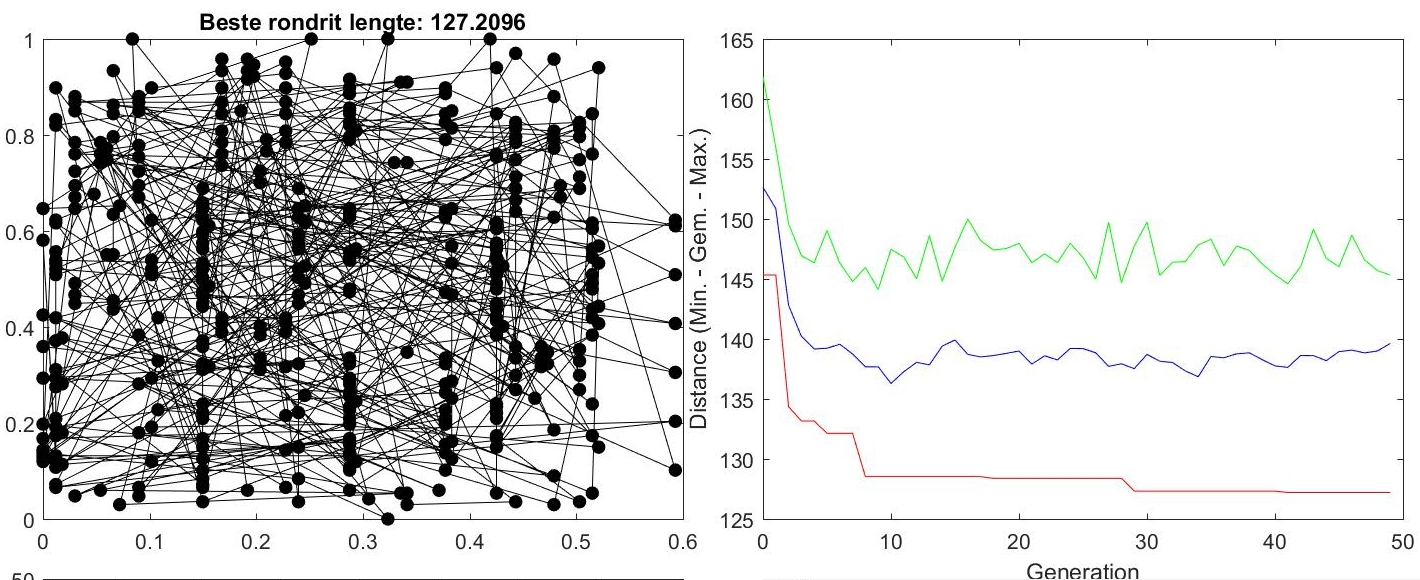
\includegraphics[width=13cm]{img/specific/order_crossover/general_1.jpg}
\end{center}

The first noticeable thing that we can observe here is that the distance
is far higher than the adjacency representation, although looking at the
time, it is better, since it takes only 6.88 seconds.\\
\\
We have the same situation that we had with the number of generations in the
previous representation, but this time with the number of individuals. While
200 was the amount with the generally lower distances, higher numbers also
performed somewhat ok. Thus we tested for 200, 1000, and 1250.\\

\text{\big[200,50,5\%,95\%,5\%\big]}
\hfill
\text{\big[1000,50,50\%,95\%,5\%\big]} \\
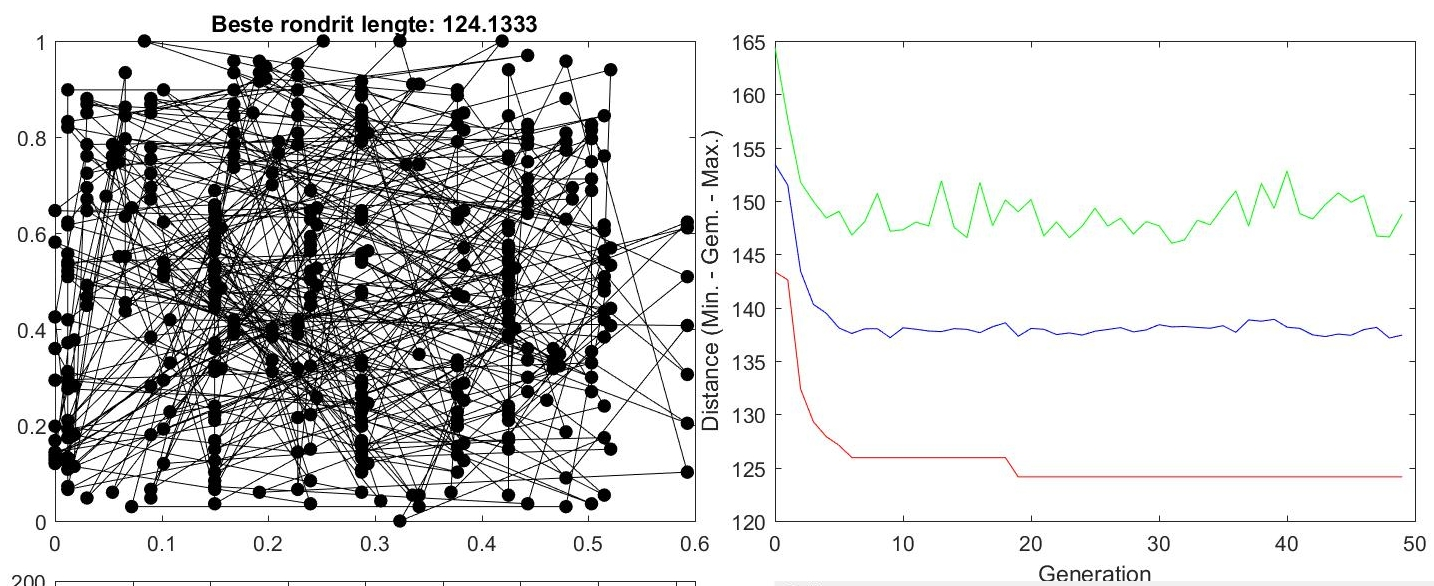
\includegraphics[width=9cm]{img/specific/order_crossover/general_2.jpg}
\hfill
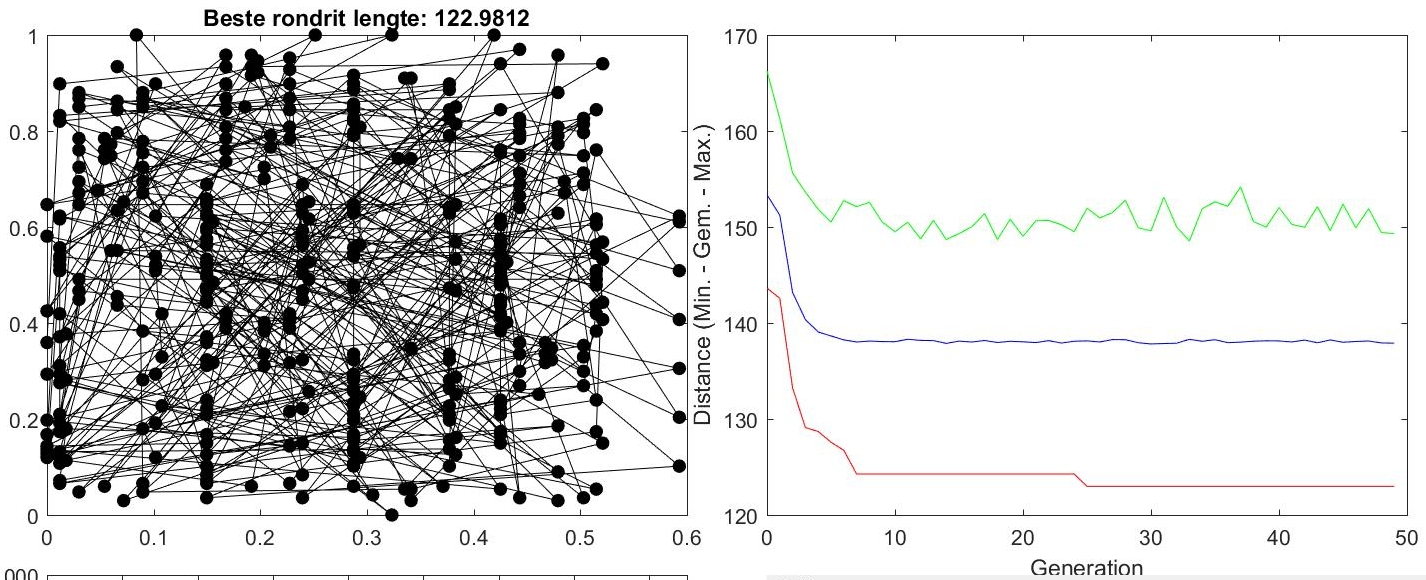
\includegraphics[width=9cm]{img/specific/order_crossover/general_3.jpg}

\begin{center}
[1250,50,5\%,95\%,5\%]\\
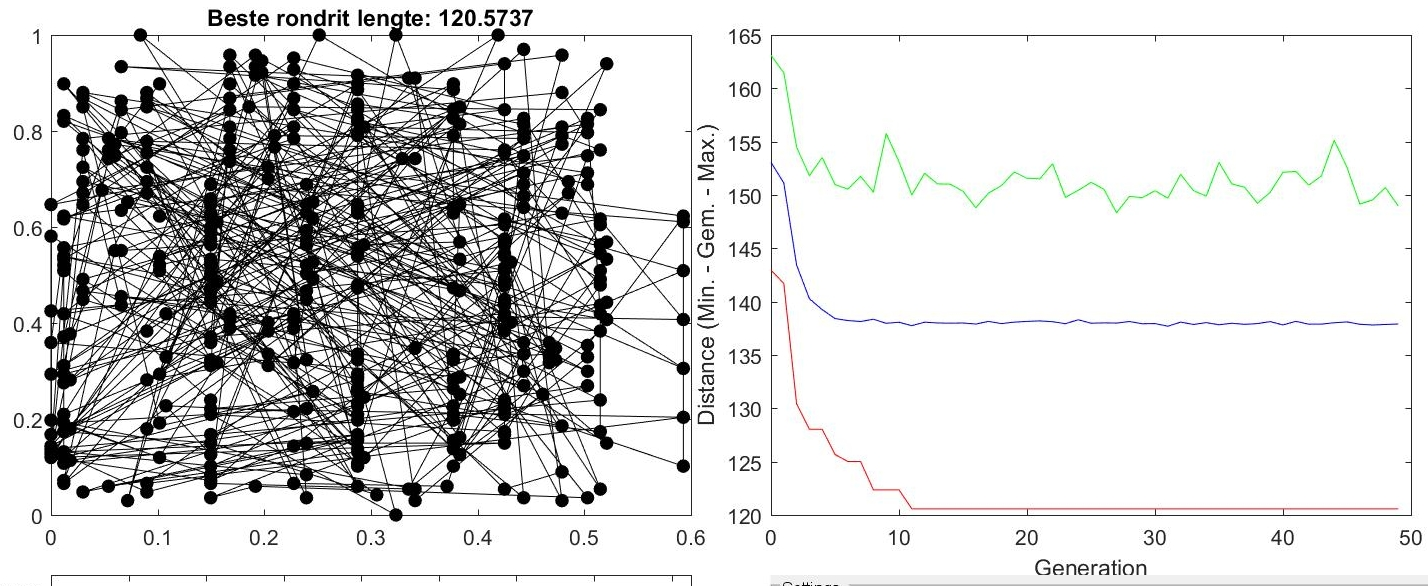
\includegraphics[width=13cm]{img/specific/order_crossover/general_4.jpg}
\end{center}

Although the change is not big, there is improvement, with each increase
of individuals. And, what's more, as it is individuals, and not
generations that we are increasnig now, there is higher cost, but not as high.
The times for the tests are 9.08, 29.44, and 37.99 seconds, being the last not
even 6 times higher. As there is the increase is the highest in the last
test (1250 individuals), and the time is not humongously high, that value
will be the one to be tested in the combined test.\\ 
\\
The general test for the number of generations revealed that the best quantity
was 200.\\
\begin{center}
[50,200,5\%,95\%,5\%]\\
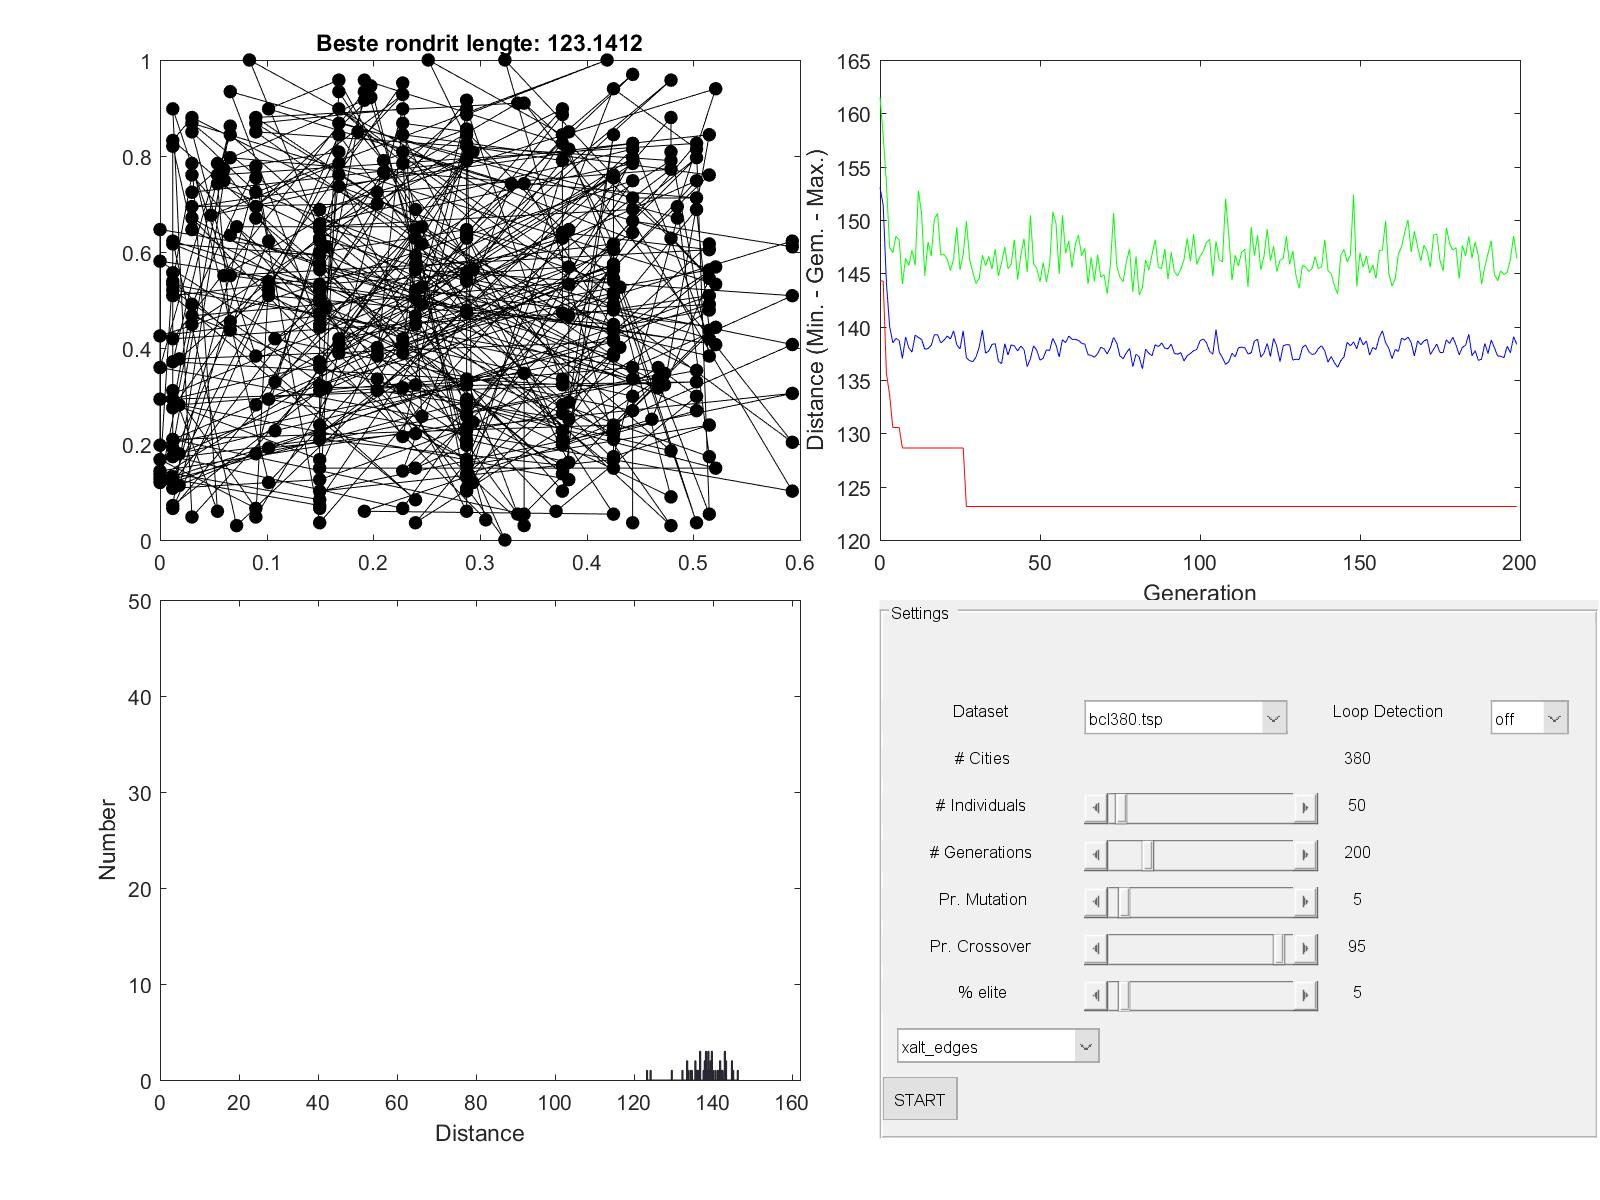
\includegraphics[width=13cm]{img/specific/order_crossover/general_5.jpg}
\end{center}

We can observe a slight improvement against the base case, 4 units of
distance. Timewise, it is much more demanding that increasing
individuals, since the test took 23.73 seconds to end, ~3.5 times more than the
base case. Any higher number of generations will only hinder the process
by making it tediously slow.\\

As happened in the previous representation tests, the general test for path
rep. showed that the value 5\% for elitism was without a doubt the best that
could be set. So, the last to test is crossover and mutation, and here comes the tricky part for this representation. We found in our general
test that no matter what the percentage for mutation or crossover was being
tested, the results were almost independant from them. So, given that the base
case already tested for a high crossover, and low mutation, the designed
tests are, for low crossover and high mutation, and for a 50|50. \\
\text{\big[50,200,5\%,10\%,90\%\big]}
\hfill
\text{\big[50,200,5\%,50\%,50\%\big]} \\
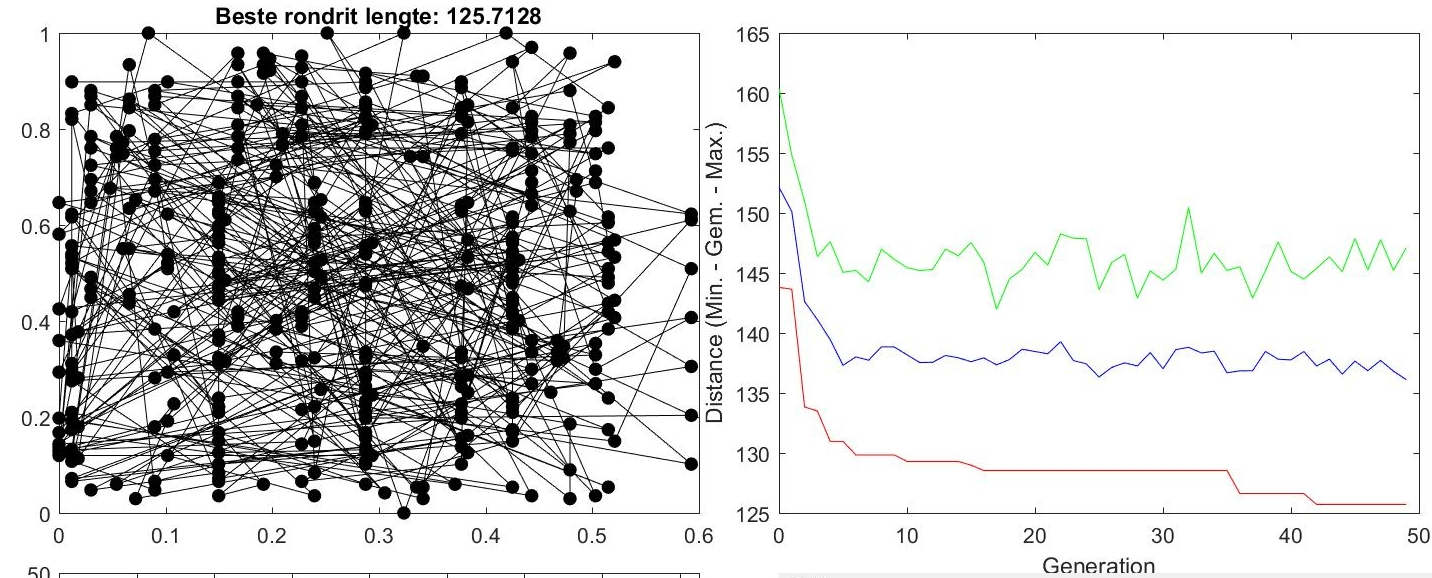
\includegraphics[width=9cm]{img/specific/order_crossover/general_6.jpg}
\hfill
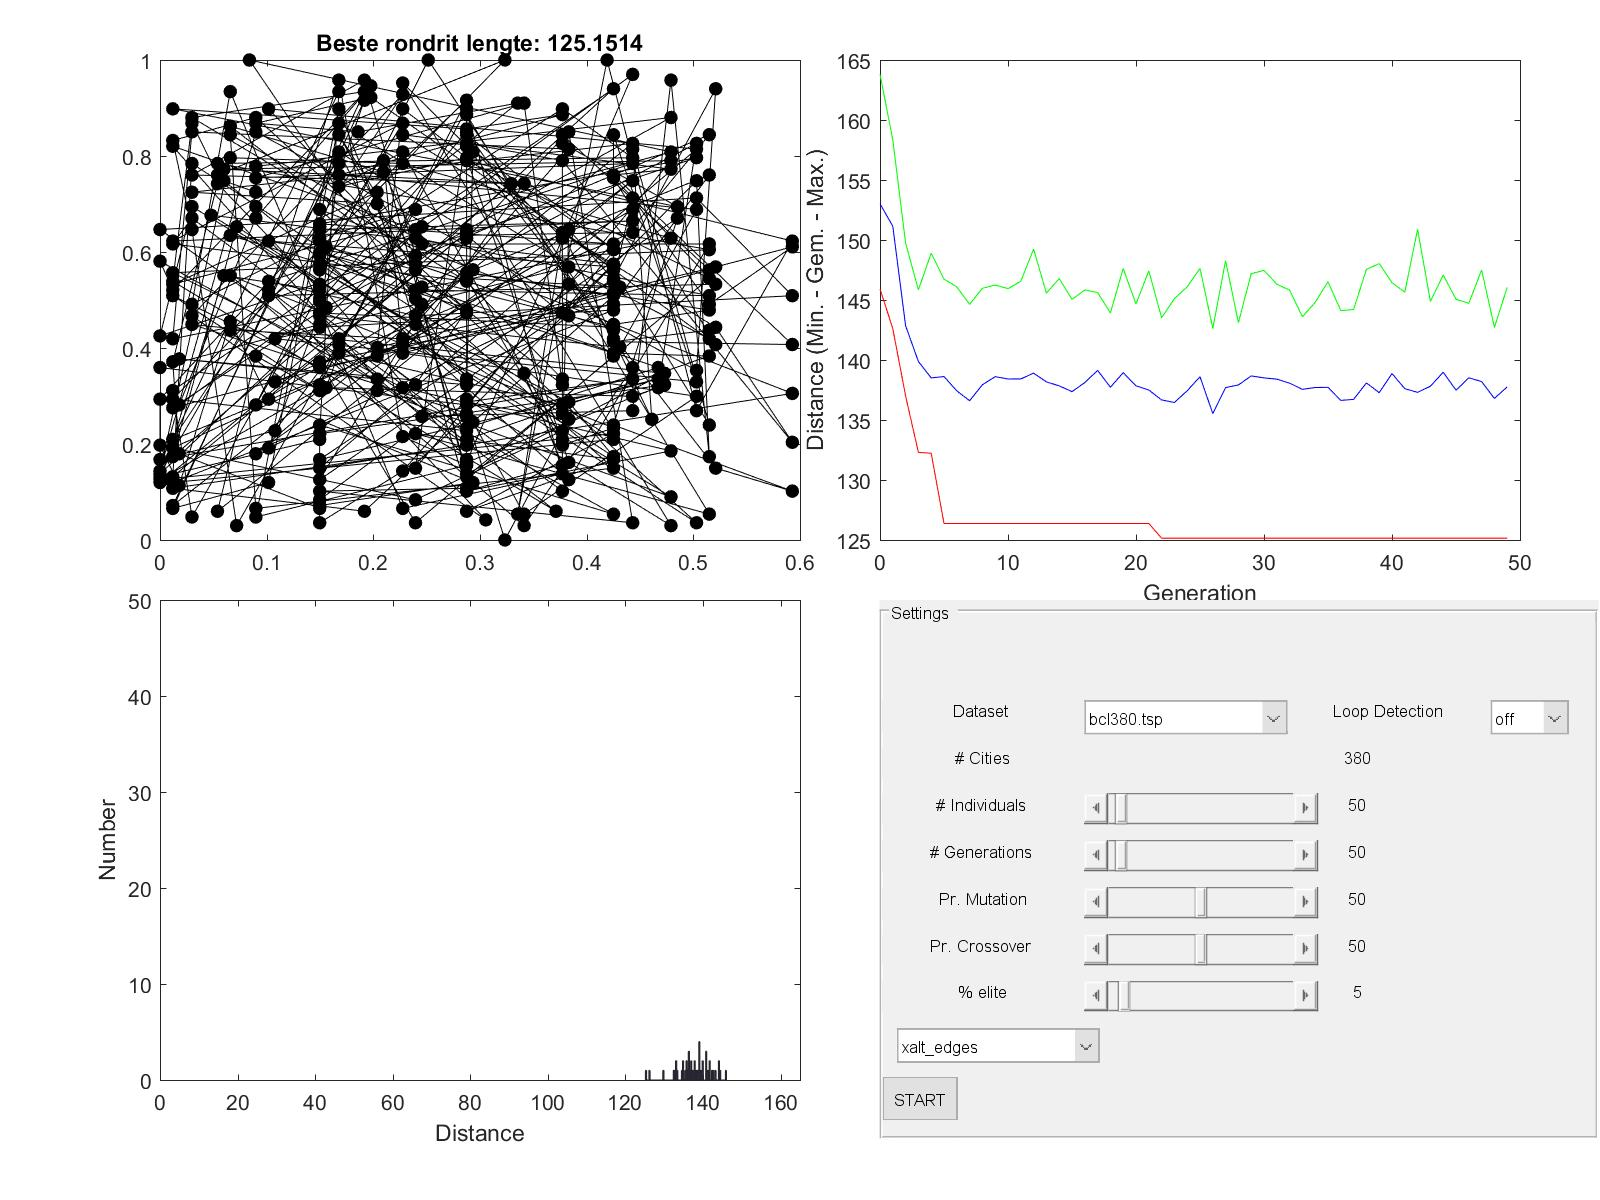
\includegraphics[width=9cm]{img/specific/order_crossover/general_7.jpg}

Although somewhat better than the base case, the result from one test to the
other differ so little that it confirms the result of the general test, stating
that, for this represention, given our implementation with our
operators, the percentage is not really relevant. But, as it's still better
than the base, and the best of the two, the percentages chosen for the combined
test are 50\%|50\%. Obviosly, as the number of indviduals or
generations did not change, the time is almost identical to the base case\\
\\
For the combined test, in hope to get the best result, this is the test made\\
\begin{center}
[1250,200,5\%,50\%,50\%]\\
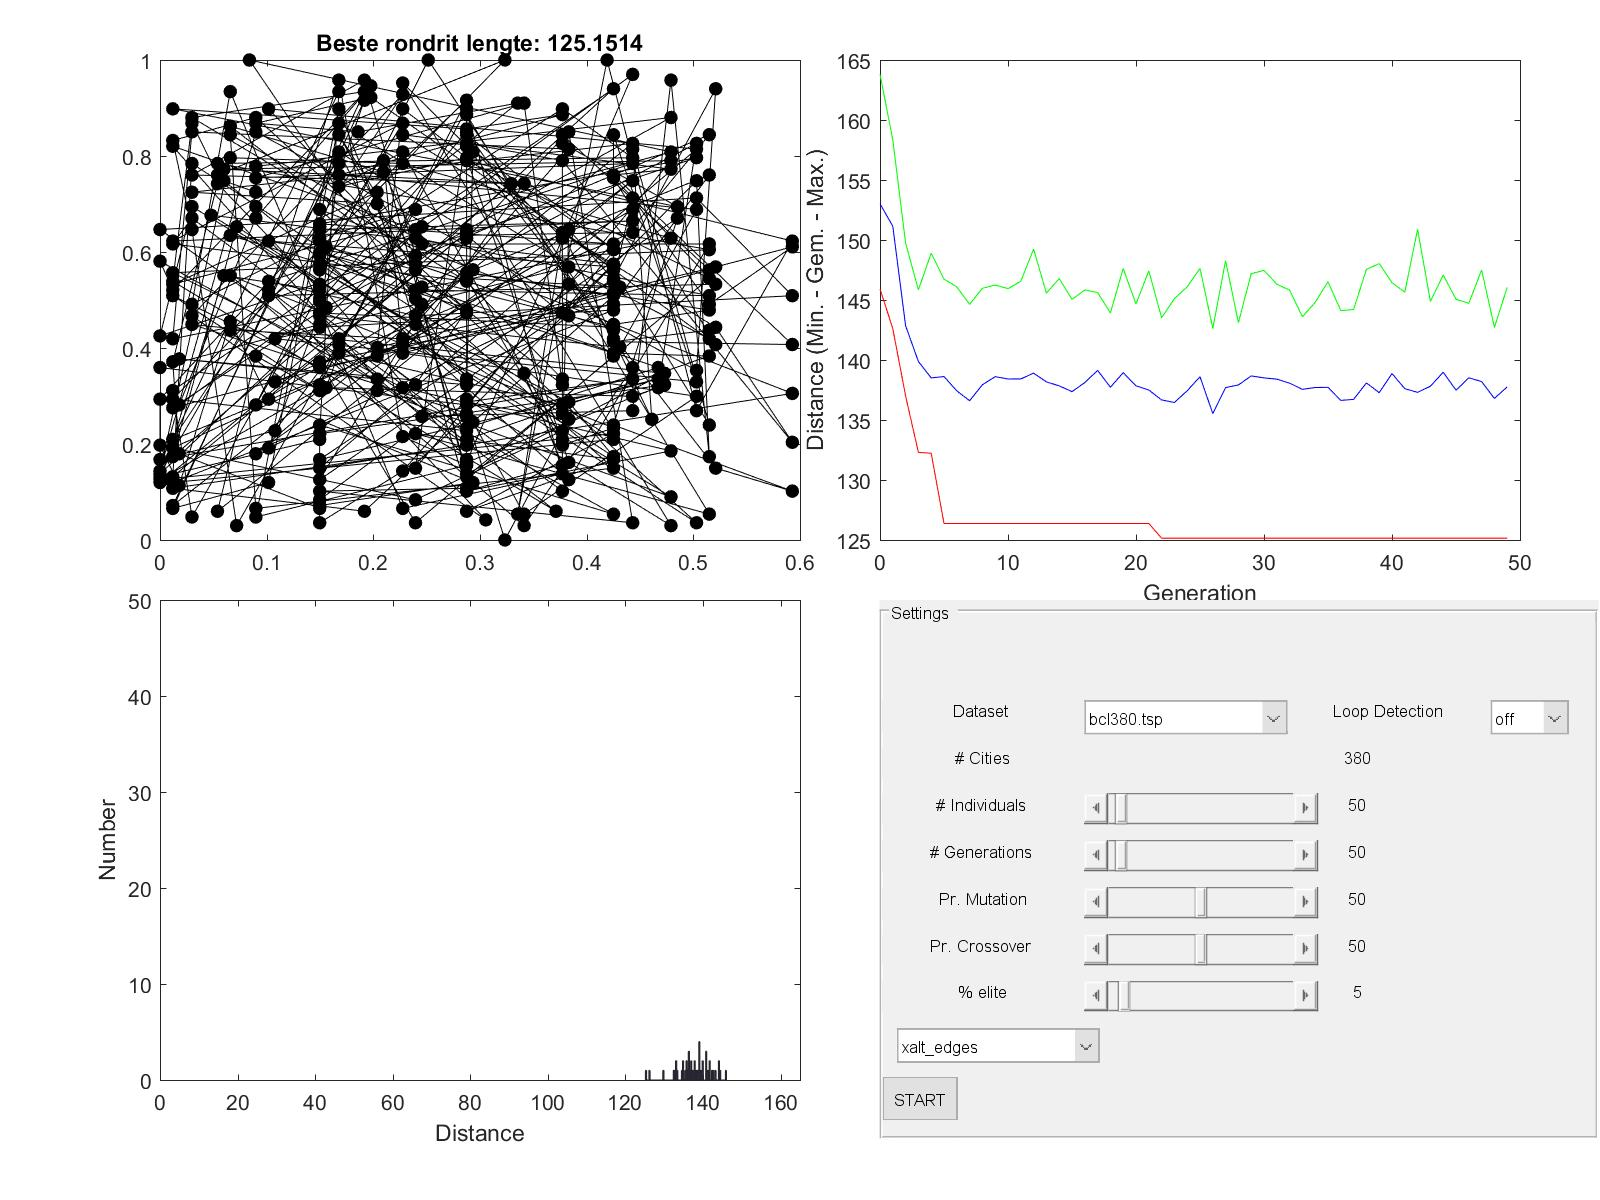
\includegraphics[width=13cm]{img/specific/order_crossover/general_7.jpg}
\end{center}

Unlike the previous combined test, the big expected improvement is nowhere
to be seen. Going from a length of 127 to 120 is just a mere ~5.2\% of
decrease. Furthermore, the combined increase of individuals and
generations, given that the former is very high, makes the test to take extremly
long compared to the base, going from 6.88 seconds to 141.02 seconds, ~20.5
times more. 

This can be due to the fact that the crossover operator favors the local
minimum and the mutation operator tries to explore new paths, but as the mutation
operator only changes the position of one number in the sequence of cities,
the exploration factor of the chosen mutation is not big enough to compete
against the exploitation of the crossover, regardless of how big the
percentage of mutation is.  



